% !TeX spellcheck = cs_CZ
%{\tikzset{external/prefix={tikz/FYZI/}}
% \tikzset{external/figure name/.add={ch02_}{}}
%---------------------------------------------------------------------------------------------------
% file fey1ch04.tex
%---------------------------------------------------------------------------------------------------
%================= Kapitola: Zachování energie =====================================================
\chapter{Zachování energie}\label{fyz:IchapII}
\minitoc
  \section{Co je to energie}
    Skončili jsme s obecným popisem věcí, a proto v této kapitole začneme podrobněji studovat různé 
    aspekty fyziky. Pro ilustraci myšlenek a způsobů argumentace používaných v teoretické fyzice 
    budeme zkoumat jeden z nejzákladnějších zákonů fyziky, \textbf{zákon zachování energie}.
    
    Existuje skutečnost nebo chceme-li \emph{zákon}, kterým se řídí všechny přírodní jevy. Pokud 
    víme, tento zákon je přesný a neexistuje z něho žádná výjimka. Je to \emph{zákon zachování 
    energie}. Říká, že existuje veličina nazývaná energií, která se nemění v průběhu mnoha změn, 
    jež podstupuje příroda. To je velmi abstraktní myšlenka, vždyť jde o matematický princip; 
    hovoří o existenci číselné veličiny, která se v průběhu procesů nemění. Není to popis 
    mechanizmu, ani něčeho konkrétního; je to jen podivuhodná skutečnost, když spočítáme nějakou 
    veličinu, pak pozorujeme, jak příroda provádí své kousky, nakonec provedeme výpočet znovu a 
    dostaneme totéž Číslo. (Něco jako střelec na černém poli, který po určitém počtu kroků - které 
    detailně neznáme - se stále nachází na černém poli. To je zákon této hry.) Protože jde o 
    abstraktní myšlenku, ilustrujme její smysl pomocí analogie.
    
    Představme si dítě, například nějakého Cipíska, který má kostky. Jsou nezničitelné, nelze je 
    rozdělit na části a všechny jsou stejné. Předpokládejme, že Cipísek má \num{28} kostek. Matka 
    ho ráno nechá i s \num{28} kostkami v pokoji a každý večer ze zvědavosti starostlivě spočítá 
    všechny kostky. Tak objeví fenomenální zákonitost - bez ohledu na to, co chlapec s kostkami 
    dělal, zůstane vždy \num{28} kostek. Takováto situace se opakuje několik dní, až jednou zůstane 
    jen \num{27} kostek. Krátké hledání však ukáže, že jedna kostka je pod kobercem, že se počet 
    kostek nezměnil. Jednoho dne se však počet kostek změnil - zůstalo jich jen \num{26}. Pečlivý 
    průzkum, který matka provedla, však ukázal, že bylo otevřené okno a tím se dostaly dvě kostky 
    ven. Jednoho dne však napočítala \num{30} kostek, což vyvolalo značné překvapení. Potom si však 
    matka uvědomila, že Cipísek měl na návštěvě kamaráda, který si s sebou přinesl své kostky a 
    několik jich u Cipíska zapomněl. Když matka vrátila přebytečné kostky, zavřela okno a nepustila 
    kamarády, všechno bylo zase v pořádku, až jednou při počítání zjistila, že je jen \num{25} 
    kostek. V pokoji byla krabice na hračky a když se matka do ní chtěla podívat, chlapec to 
    nechtěl dovolit a dal se do křiku. Matka však byla velmi zvědavá a dost vynalézavá, a proto si 
    vymyslela trik. Věděla, že každá kostka váží \SI{100}{\gram}, a tak zvážila krabici, když bylo 
    všech \num{28} kostek venku. Zjistila, že váží \SI{500}{\gram}, a proto při další kontrole 
    kostek zvážila opět krabici, odečetla \SI{500}{\gram} a dělila stem. Tak objevila zákonitost
    \begin{equation*}
      \renewcommand{\arraystretch}{0.8}
        \begin{pmatrix} 
          \text{\footnotesize{počet}}   \\
          \text{\footnotesize{kostek}}  \\
          \text{\footnotesize{venku}}
        \end{pmatrix}   +
      \frac{
        \begin{pmatrix}
          \text{\footnotesize{hmotnost}}  \\
          \text{\footnotesize{krabice}}
        \end{pmatrix}
        - \SI{500}{\gram}}{ \SI{100}{\gram}} = 
      \text{konst.}
    \end{equation*}
    
    Později se objevily nové odchylky, ale ukázalo se, že špinavá voda ve vaně změnila svou 
    hladinu. Dítě házelo kostky do vody a matka je tam nemohla vidět, neboť voda byla špinavá. 
    Přidáním dalšího členu do vzorce však zjistila, kolik kostek je ve vodě. Protože původní výška 
    vody byla \SI{15}{\cm} a každá kostka zvedala hladinu o \SI{0.5}{\cm}, nový vzorec má tvar
    \begin{equation*}
        \begin{pmatrix} 
          \text{\footnotesize{počet}}   \\
          \text{\footnotesize{kostek}}  \\
          \text{\footnotesize{venku}}
        \end{pmatrix}
       +
      \frac{
            \begin{pmatrix}
              \text{\footnotesize{hmotnost}}  \\
              \text{\footnotesize{krabice}}
            \end{pmatrix}
        - \SI{500}{\gram}}{ \SI{100}{\gram}} +
      \frac{
            \begin{pmatrix}
              \text{\footnotesize{výška}}  \\
              \text{\footnotesize{hladiny}}
            \end{pmatrix}
        - \SI{15}{\cm}}{ \SI{0.5}{\cm}} = 
      \text{konst.}
    \end{equation*}
    Při postupném narůstání složitosti svého světa našla matka celou řadu členů odpovídajících 
    počtu kostek nacházejících se na místech, do nichž nesměla nahlédnout. Tak našla komplexní 
    vzorec pro veličinu, kterou je třeba vypočítat a která v podmínkách jejího světa zůstává stálá.
    
    Čím je tento příklad podobný zákonu zachování energie? Musíme udělat jednu důležitou abstrakci 
    musíme si \emph{odmyslet kostky}. Odstraníme-li první členy v obou rovnicích, zjistíme, že 
    počítáme víceméně abstraktní věci. Podobnost spočívá především v tom, že počítáme-li energii, 
    dostáváme se do situace, že někdy část energie odchází ze systému a někdy zase do systému 
    přichází. Abychom ověřili zákon zachování energie, musíme dávat pozor, aby nic nepřišlo ani 
    neodešlo. Dále, energie má mnoho různých forem a pro každou z nich máme zvláštní vzorec. Jsou 
    to: \emph{gravitační energie}, \emph{kinetická energie}, \emph{tepelná energie}, 
    \emph{elastická energie}, \emph{elektrická energie}, \emph{chemická energie}, \emph{radiační 
    energie}, \emph{jaderná energie}, \emph{energie vázaná na hmotnost}. Když sčítáme příspěvky od 
    jednotlivých energií, součet se nezmění, nebude-li nějaká energie dodána nebo odebrána.
    
    Je důležité si uvědomit, že současná fyzika vlastně neví, co je to energie. Nepředstavujeme si, 
    že by se energie vyskytovala v určitém počtu malých kapiček. Tak to není. Existují však vztahy 
    pro výpočet určité číselné veličiny a při sčítání všech příspěvků dostáváme „\num{28}“ - vždy 
    stejné číslo. Je to abstraktní věc v tom smyslu, že to neříká nic o mechanizmu nebo 
    \emph{příčinách} jednotlivých vztahů.
    
  \section{Gravitační potenciální energie}
    O zákonu zachování energie můžeme mluvit až poté, co budeme znát vyjádření všech forem energie. 
    Nejdříve se budeme zajímat o vyjádření gravitační energie v blízkosti zemského povrchu a vztah 
    pro tuto energii odvodíme způsobem, který nemá nic společného s historií, ale byl vymyšlen 
    speciálně pro tuto kapitolu, abychom zdůraznili tu pozoruhodnou skutečnost, že důkladným 
    uvažováním můžeme o přírodě mnoho poznat i z malého množství faktů. Tento postup je ilustrací 
    práce teoretických fyziků. Za vzor slouží vynikající argumentace Carnota o účinnosti parních 
    strojů. Naším cílem není ani tak výsledek (\ref{FYZ:eq056}), který již znáte, ale možnost jeho 
    získání teoretickým uvažováním.

    \begin{wrapfigure}[8]{r}{5cm}  %\ref{fyz:fig048}
      \centering
      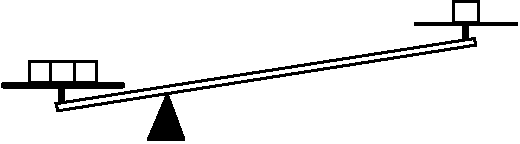
\includegraphics[width=0.9\linewidth]{fyz_fig048.pdf}
      \caption{Jednoduchý stroj na zvedání (\cite[s.~52]{Feynman01})}
      \label{fyz:fig048}
    \end{wrapfigure}
    Mějme zařízení na zvedání, jež má tu vlastnost, že zvedá jedno závaží spouštěním druhého. 
    Přitom předpokládejme, že v případě tohoto zařízení neexistuje něco takového jako je 
    \emph{neustálý pohyb}. (Fakt, že vůbec neexistuje neustálý pohyb, je obecným tvrzením zákona 
    zachování energie.) Při definování neustálého pohybu musíme být opatrní. Udělejme to nejdříve 
    pro zvedací zařízení. Jestliže jsme při zvedání a spouštění množství závaží dostali zařízení do 
    původního stavu a zjistíme, že čistým výsledkem je \emph{zvednutí určité hmotnosti}, pak máme 
    zařízení na stálý pohyb, protože tuto zvednutou hmotnost můžeme použít jako pohon něčeho 
    jiného. Přitom musí být splněna podmínka, že zařízení zvedající závaží se přivádí přesně do 
    původního stavu a dále, že zařízení je úplně uzavřené, že nezískává energii na zvedání závaží z 
    nějakého vnějšího zdroje - tak jak to bylo v případě, kdy Cipískovi nechal v pokoji kostky jeho 
    přítel.
    
    Velmi jednoduché zařízení na zvedání je znázorněno na obr. \ref{fyz:fig048}. Toto zařízení 
    zvedá závaží sestávající ze tří jednotek. Tři jednotky položíme na jednu misku a jednu jednotku 
    na druhou. Abychom zařízení skutečně uvedli do činnosti, musíme z levé misky odebrat část 
    závaží. Naopak, můžeme zvedat jednotkové závaží spouštěním závaží sestávajícího ze tří jednotek 
    takovým trikem, že z jednotkového závaží trochu ubereme. Uvědomujeme si, samozřejmě, že v 
    případě \emph{skutečných} vah musíme něco dodat, abychom je uvedli do činnosti. To budeme 
    \emph{dočasné} ignorovat. Ideální zařízení, která však neexistují, si nevyžadují nic 
    dodatečného. Zařízení, které skutečně používáme, může být v určitém smyslu \emph{téměř} vratné: 
    tj. zvedne-li hmotnost tří jednotek tím, že nechá klesnout hmotnost jedné jednotky, pak také 
    stejně zvedne hmotnost jedné jednotky tím, že nechá klesnout hmotnost tří jednotek.
    
    Představme si, že existují dva druhy strojů. Takové, které \emph{nejsou} vratné (k nim patří 
    všechny skutečné stroje) a také takové, které \emph{jsou} vratné (samozřejmě nedosažitelné bez 
    zřetele na pečlivost, jíž věnujeme návrhu jejich ložisek, pák atd.). Předpokládejme však, že 
    existuje takové zařízení - vratný stroj - které spouští jednotkové závaží (kilogramu nebo jiné 
    jednotky) o jednotkovou vzdálenost a současně zvedá tři jednotková závaží. Nazveme ho vratným 
    strojem, strojem \texttt{A}. Předpokládejme, Že tento speciální vratný stroj zvedá tři 
    jednotková závaží o výšku \emph{X}. Dále předpokládejme, že máme jiné zařízení, stroj 
    \texttt{B}, který nemusí být vratný, a ten rovněž nechá klesnout jednotkové závaží o 
    jednotkovou vzdálenost, ale zvedne tři jednotková závaží o výšku \emph{Y}. Lze dokázat, že 
    \emph{Y} není větší než \emph{X} tj. že není možné sestrojit zařízení, které by zvedalo závaží 
    výše než ho zvedá vratný stroj. Řekněme si proč. Předpokládejme, že \emph{Y} je větší než 
    \emph{X}. Vezměme jednotkové závaží a nechme ho klesnout o jednotkovou výšku na stroji 
    \texttt{B}, což způsobí zvednutí tří jednotkových závaží o výšku \emph{Y}. Potom můžeme závaží 
    spustit z výšky \emph{Y} do výšky \emph{X}, získat tak výkon „zadarmo“ a použít vratný stroj 
    \texttt{A} při zpětném chodu ke spuštění tří jednotkových závaží o výšku \emph{X} a zvednutí 
    jednotkového závaží o jednotkovou výšku. To vrátí jednotkové závaží do původního stavu a oba 
    stroje budou připraveny k opětovnému použití! Kdyby bylo \emph{Y} větší než \emph{X}, dostali 
    bychom neustálý pohyb, ale ten považujeme za nemožný. Z toho usuzujeme, že \emph{Y} \emph{není 
    větší než} \emph{X} takže ze všech strojů je nejlepší vratný stroj.
    
    Je vidět, že všechny vratné stroje musejí zvedat \emph{přesně do stejné výšky}. Předpokládejme, 
    že i stroj \texttt{B} by byl skutečně vratný. Tvrzení, že \emph{Y} není větší než \emph{X}, 
    zůstává, samozřejmě, v platnosti, ale tvrzení můžeme obrátit, použijeme-li stroje v opačném 
    pořadí a dokážeme, že \emph{X} není větší než \emph{Y}. To je zajímavý poznatek, neboť umožňuje 
    zkoumat výšku, do níž různé stroje zvednou závaží, bez ohledu na jejich vnitřní mechanizmus. 
    Ihned víme, že velmi složitá soustava pák, která zvedá tři jednotková závaží do určité výšky za 
    současného poklesu jednotkového závaží o jednotkovou výšku, nebude lepší, spíše horší než 
    jednoduchá páka konající totéž, když je v podstatě vratná. Je-li složitá soustava vratná, víme 
    přesně do jaké výšky zvedá závaží. Závěrem je možné říci, že každý vratný stroj, bez ohledu na 
    způsob jeho činnosti, který spouští jeden kilogram o jeden metr a zvedá tři kilogramy, zvedá 
    tuto hmotnost vždy o stejnou výšku \emph{X}. To je obecný zákon, který má široké užití. Další 
    otázkou samozřejmě je, jak velké je \emph{X}?

    \begin{figure}[ht!]  % \ref{fyz:fig049}
      \centering
      \begin{tabular}{cc}
        \subfloat[ ]{\label{fyz:fig049a}
          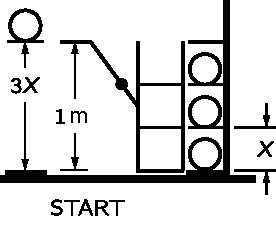
\includegraphics[width=0.4\linewidth]{fyz_fig049a.pdf}}
        \hspace{0.1\linewidth}                                                       &
        \subfloat[ ]{\label{fyz:fig049b}
          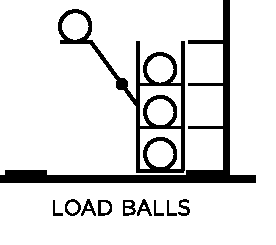
\includegraphics[width=0.4\linewidth]{fyz_fig049b.pdf}}                   \\
        \subfloat[ ]{\label{fyz:fig049c}
          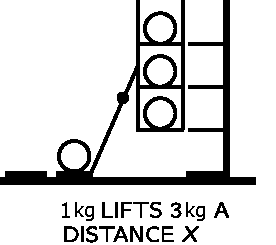
\includegraphics[width=0.4\linewidth]{fyz_fig049c.pdf}}
        \hspace{0.1\linewidth}                                                       &
        \subfloat[ ]{\label{fyz:fig049d}
          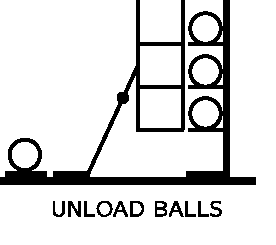
\includegraphics[width=0.4\linewidth]{fyz_fig049d.pdf}}                   \\
        \subfloat[ ]{\label{fyz:fig049e}
          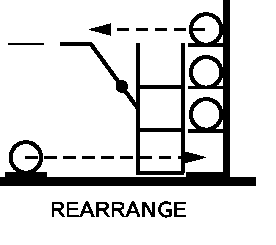
\includegraphics[width=0.4\linewidth]{fyz_fig049e.pdf}}
        \hspace{0.1\linewidth}                                                       &
        \subfloat[ ]{\label{fyz:fig049f}
          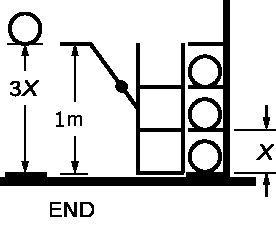
\includegraphics[width=0.4\linewidth]{fyz_fig049f.pdf}}
      \end{tabular}
      \caption{Vratný stroj: a) počáteční poloha; b) nakládáni míčků; c) 1 kg zvedá 3 kg do výšky 
               \emph{X}; e) přeskupení  d) vykládáni míčků; e) konečná poloha 
               \cite[s.~53]{Feynman01}}
      \label{fyz:fig049}
    \end{figure}
    
    Předpokládejme, že máme vratný stroj, který zprostředkuje zvednutí tří jednotkových závaží do 
    výšky \emph{X} pomocí jednotkového závaží. Tři míčky umístíme do pevných polic tak, jak 
    znázorňuje obr. \ref{fyz:fig049}. Jeden míček stojí na stojanu ve výšce jednoho metru nad zemí. 
    Zařízení může zvednout tři míčky tím, že jeden míček klesne o jeden metr. Uspořádání pokusu je 
    takové, že police, ve kterých jsou míčky, jsou ve vertikálním směru vzájemně vzdálené o 
    \emph{X} a plošina, která bude míčky zvedat, má také vertikálně uspořádané přihrádky vzájemně 
    vzdálené o \emph{X} (a). Nejdříve překutálíme míčky horizontálně z polic do přihrádek (b), 
    přičemž nepředpokládáme změnu energie, neboť se nemění výška.

    Pak se uvede do činností vratný stroj: spustí jeden míček až k podlaze a zvedne plošinu o 
    vzdálenost \emph{X} (c). Zvedací plošinu jsme navrhli tak důmyslně, že její přihrádky stojí 
    opět proti policím. Míčky pak odkutálíme do polic (d). Po odkutálení míčků můžeme stroj vrátit 
    do jeho původního stavu (e). Tak jsme dostali tři míčky do horních polic a jeden na podlahu. 
    Zvláštností je, že jsme vlastně dva z nich vůbec nezvedali, neboť v policích 2 a 3 byly i 
    předtím. Výsledný efekt tedy je, že se zvedl \emph{jeden míček} do výšky \emph{3X} Kdyby 
    \emph{3X} přesahovalo jeden metr, mohli bychom dát míček níže, aby se stroj dostal do původního 
    stavu (f), a mohl znovu začít činnost. Proto \emph{3X} nemůže přesáhnout jeden metr, neboť v 
    opačném případě bychom měli perpetuum mobile. Podobným způsobem můžeme dokázat, že \emph{jeden 
    metr nemůže převýšit 3X}, stačí, když necháme stroj pracovat naopak, jde-li o vratný stroj. 
    \emph{3X} tedy není ani více, ani méně než jeden metr a tímto zdůvodněním jsme zjistili, že 
    \(X= 1/3\) metru. Zobecnění je jasné: klesne-li při činnosti vratného stroje jednokilogramové 
    závaží o určitou vzdálenost, zvedne stroj \emph{p-}kilogramové závaží o vzdálenost \(1/p\). 
    Jiný způsob vyjádření výsledku je následující: tři kilogramy vynásobené výškou zdvihu, v našem 
    případě \emph{X}, jsou rovny jednomu kilogramu vynásobenému velikostí poklesu, v našem případě 
    jedním metrem. Vezmeme-li tíhy všech těles a vynásobíme je výškami, v nichž se nacházejí, pak 
    necháme pracovat stroj a násobíme opět všechny tíhy výškami, \emph{nenastane změna}. (Musíme 
    zobecnit příklad, v němž jsme pohybovali jen jedním závažím na případ, kdy snížením jednoho 
    zvedáme několik různých závaží - ale to je jednoduché).
    
    Součet tíh násobených výškami nazýváme \emph{gravitační potenciální energií}- energií, kterou 
    má objekt díky své poloze v prostoru vzhledem k Zemi. Vyjádření gravitační energie, nejsme-li 
    příliš vzdáleni od Země (síla slábne se vzrůstající výškou), je následující:
    \begin{equation}\label{FYZ:eq056}
      \renewcommand{\arraystretch}{0.8}
      \left(
        \begin{array}{c}
          \text{gravitační potenciální}  \\
          \text{energie objektu}
        \end{array}
      \right) =
      \text{tíha} \cdot \text{výška}.
    \end{equation}

    Je to krásný způsob důkazu. Zůstává však otázka, zda není nepravdivý. (Nakonec, příroda se 
    nemusí chovat podle našeho důkazu.) Co kdyby perpetuum mobile přece jen existovalo? Některé z 
    našich předpokladů mohou být nesprávné, nebo jsme se mohli dopustit chyby při argumentaci, 
    takže je vždy potřebná zkouška. Experiment však ukazuje, že tento zákon je správný.
    
    Obecný název pro energii, která souvisí s polohou vůči něčemu jinému, je potenciální energie. V 
    našem speciálním případě ji nazýváme gravitační potenciální energií. Máme-li místo gravitačních 
    sil co činit s elektrickými silami, proti nimž konáme práci oddalováním jedněch nábojů od 
    druhých soustavou pák, mluvíme o elektrické potenciální energii. Obecným principem je, že změna 
    energie je vyjádřena součinem síly a vzdálenosti, na které tato síla působí - to platí pro 
    změnu energie obecně:
    \begin{equation}\label{FYZ:eq057}
      \renewcommand{\arraystretch}{0.8}
      \text{změna energie} = 
      \text{síla} \cdot
      \left(
        \begin{array}{c}
          \text{vzdálenost na}  \\
          \text{kterou síla působí}
        \end{array}
      \right)
    \end{equation}

    \begin{wrapfigure}[12]{r}{5cm}  %\ref{fyz:fig051}
      \centering
      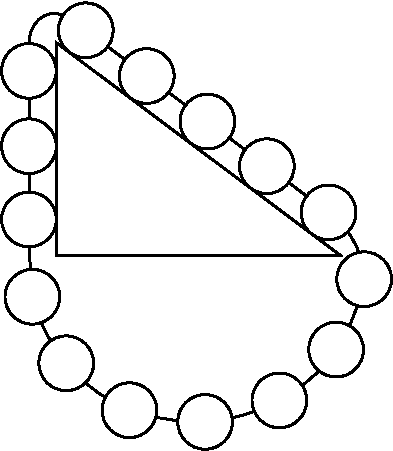
\includegraphics[width=0.6\linewidth]{fyz_fig051.pdf}
      \caption{Stevinův epitaf (\cite[s.~55]{Feynman01})}
      \label{fyz:fig051}
    \end{wrapfigure}
    V průběhu tohoto kurzu se vrátíme k mnoha z jiných druhů energie.

    Princip zachování energie nám v řadě případů velmi pomáhá při úvahách o tom, co se se systémem 
    stane. Na střední škole jsme se učili mnoho zákonů o kladkách a pákách použitých různými 
    způsoby. Teď vidíme, že tyto „zákony“ představují \emph{vlastně jediný zákon} a není proto 
    třeba pamatovat si \num{75} pravidel k jeho vyjádření. Jednoduchým příkladem je \emph{hladká 
    nakloněná rovina}, pro kterou jsme šťastně zvolili trojúhelník s poměrem stran 
    \num{3}:\num{4}:\num{5} (obr. \ref{fyz:fig049}). Na nakloněnou rovinu s kladkou zavěsíme závaží 
    jednoho kilogramu a na druhou stranu kladky těleso o hmotnosti \(m\). Zajímá nás, jak velké 
    musí být \(m\), aby vyvážilo jeden kilogram na nakloněné rovině. Jak to můžeme vypočítat? 
    Říkáme-li, že soustava je právě vyvážená, pak je vratná, a proto se může pohybovat nahoru a 
    dolů. Můžeme si představit následující situaci. V počátečním stavu (a) je kilogramové závaží 
    dole a těleso o hmotnosti \(m\) nahoře. Sklouzlo-li \(m\) vratným způsobem dolů, je kilogramové 
    závaží nahoře a těleso se šikmo vzdálilo o pět metrů od roviny, v níž bylo původně (b). Zvedli 
    jsme kilogramové závaží jen o tři metry a těleso o hmotnosti \(m\) klesalo po dráze pěti metrů; 
    proto \(m = 3/5\) kilogramu. Všimněte si, že v naší úvaze jsme použili jen zákon zachování 
    energie a nebrali jsme v úvahu složky sil. Naše šikovnost je však jen relativní. Dedukci je 
    možné provést ještě důmyslnějším způsobem, na který přišel \emph{Stevinus} a který je vyrytý na 
    jeho náhrobním kameni. Obr. \ref{fyz:fig050} vysvětluje, že to musí být 3/5 kilogramu, neboť 
    řetěz se nebude

    \begin{figure}[ht!]  %\ref{fyz:fig050}
      \centering
      \begin{tabular}{cc}
        \subfloat[ ]{\label{fyz:fig050a}
          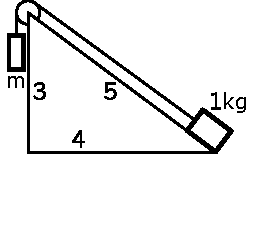
\includegraphics[width=0.2\textwidth]{fyz_fig050a.pdf}}
        \hspace{0.1\linewidth}                                                       &
        \subfloat[ ]{\label{fyz:fig050b}
          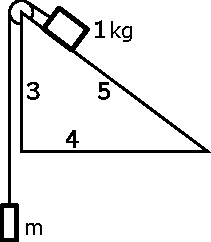
\includegraphics[width=0.17\textwidth]{fyz_fig050b.pdf}}
      \end{tabular}
      \caption{Nakloněna rovina (\cite[s.~55]{Feynman01})}
      \label{fyz:fig050}
    \end{figure}
      
    \begin{figure}[ht!]  %\ref{fyz:fig052}
      \centering
      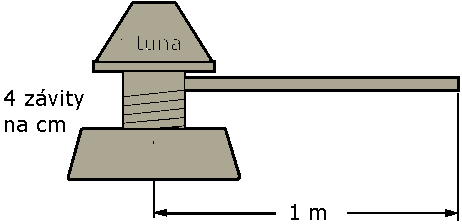
\includegraphics[width=0.7\linewidth]{fyz_fig052.pdf}
      \caption{Hever (\cite[s.~55]{Feynman01})}
      \label{fyz:fig052}
    \end{figure}
    Ilustrujme nyní energetický princip na složitějším problému, na \textbf{šroubovém zvedáku} 
    znázorněném na obr. \ref{fyz:fig052}. K otáčení šroubu slouží rukojeť dlouhá \SI{1}{\m} a šroub 
    má \num{4} závity na \num{1} centimetr. Zajímá nás, jakou silou musíme působit na rukojeť, 
    abychom zvedli břemeno o hmotnosti \num{1} tuny. Chceme-li zvednout tunu o jeden centimetr, 
    musíme otočit rukojeť čtyřikrát. Při jednom okružním pohybu opíše konec rukojeti dráhu 
    přibližně \SI{628}{\cm}. Rukojeť tedy musí projít \SI{2512}{\cm}. Použijeme-li různé kladky 
    apod., budeme zvedat jednu tunu neznámým malým závažím o hmotnosti \(m\) působícím na konec 
    rukojeti. Tak zjistíme, že \(m\) je asi \SI{4}{\kg}. Takový je následek zákona zachování 
    energie.

    Vezměme si teď ještě složitější příklad znázorněný na obr. \ref{fyz:fig053}. Tyč dlouhá 
    \SI{2}{\m} je upevněna na jednom konci. Uprostřed tyče je \num{30} kilogramové a ve vzdálenosti 
    \SI{0.5}{\m} od opory je \num{50} kilogramové závaží. Jak velkou silou musíme zvedat konec 
    tyče, aby byla vyvážená, neuvažujeme-li její vlastní hmotnost?
    
    \begin{figure}[ht!]  %\ref{fyz:fig053}
      \centering
      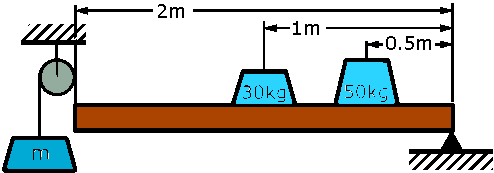
\includegraphics[width=0.7\linewidth]{fyz_fig053.pdf}
      \caption{Zatížená tyč podepřená na jednom konci (\cite[s.~56]{Feynman01})}
      \label{fyz:fig053}
    \end{figure}
    
    Předpokládejme, že na jeden konec jsme dali kladku, na níž visí závaží. Jak velkou hmotnost 
    \(m\) má mít závaží, aby nastala rovnováha? Představme si, že závaží klesne o libovolnou 
    vzdálenost. Abychom si situaci zjednodušili, předpokládejme, že klesne o \SI{10}{cm}. Ptáme se, 
    jak se zvednou uvedená závaží. Střed tyče se zvedne o \SI{5}{\cm} a bod, který je ve čtvrtině 
    vzdálenosti od opory se zvedne o \SI{2.5}{\cm}. Potom princip, že součet součinů výšek a 
    hmotností těles se nemění, říká: hmotnost \(m\) krát \SI{10}{\cm} dolů, plus \SI{30}{\kg} krát 
    \SI{5}{\cm} nahoru, plus \SI{50}{\kg} krát \SI{2.5}{\cm} nahoru je roven nule
    
    \begin{equation*}
       -\SI{10}{\m} + \num{5}\times\num{30} + \num{2.5}\times\num{50} = \num{0}, 
       \qquad m = \SI{27.5}{\kg}.
    \end{equation*}
    K vyvážení tyče je tedy třeba závaží o hmotnosti \SI{27.5}{\kg}. Takovým způsobem můžeme 
    produkovat zákony „rovnováhy“ - statiku složitých mostních konstrukcí apod. Tento přístup se 
    nazývá \textbf{princip virtuální práce}, neboť v úvahách jsme si museli \emph{představit}, že 
    systém se trochu pohybuje - ačkoli se ve \emph{skutečnosti} nepohybuje, nebo je dokonce 
    \emph{nepohyblivý}. Tento nepatrný neskutečný pohyb jsme použili proto, abychom mohli aplikovat 
    princip zachování energie.

  \section{Kinetická energie}
    Pro objasnění jiného druhu energie uvažujme kyvadlo (obr. \ref{fyz:fig054}). Když kuličku 
    vychýlíme a pak uvolníme, bude se kývat z jedné strany na druhou. Po dobu svého pohybu z krajní 
    polohy do středu ztrácí výšku. Kam se poděje potenciální energie? Gravitační energie mizí v 
    dolní poloze, ale těleso opět stoupá vzhůru. Gravitační energie musela přejít do jiné podoby. 
    Je zřejmé, že příčinou opětovného vzestupu je \emph{pohyb} a tak se gravitační energie 
    přeměnila v dolním bodě na nějakou jinou formu.
    
    \begin{figure}[ht!]  %\ref{fyz:fig054}
      \centering
      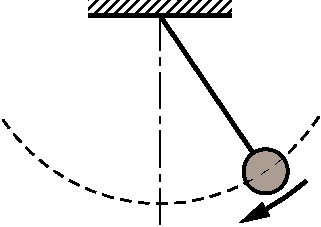
\includegraphics[width=0.5\linewidth]{fyz_fig054.pdf}
      \caption{Kyvadlo (\cite[s.~56]{Feynman01})}
      \label{fyz:fig054}
    \end{figure}
    Musíme odvodit vztah pro energii pohybu. Připomeneme-li si naše úvahy o vratných strojích, je 
    nám jasné, že při pohybu v nejnižším bodě musí být množství energie, které umožňuje kuličce 
    kyvadla dosahovat určité výšky a které nezávisí na \emph{mechanizmu}, jímž se vzestup 
    uskuteční, ani na \emph{dráze}, po níž bude kulička stoupat. Tak dostáváme vztah ekvivalence, 
    podobný vztahu, který jsme odvodili pro dětské kostky. Jednoduchým způsobem najdeme jiný vztah 
    pro vyjádření energie. Kinetická energie dole je rovna součinu tíhy \(G\) a výšky \(h\), jíž 
    může kulička v závislosti na rychlosti dosáhnout: \(W_k=G\cdot h\). Co potřebujeme, je vztah, 
    který by určil výšku pomocí pravidla souvisejícího s pohybem předmětů. Uvedeme-li nějaké těleso 
    do pohybu určitou rychlostí, směřující řekněme přímo nahoru, pak dosáhne určité výšky; zatím 
    nevíme jaké, ale tato výška závisí na rychlosti a lze ji vypočítat. Abychom našli vztah pro 
    kinetickou energii předmětu, který se pohybuje rychlostí \(v\), musíme vypočítat výšku, jíž 
    může dosáhnout a násobit ji tíhou tělesa. Brzy zjistíme, že vztah můžeme zapsat takto:
    \begin{equation}\label{FYZ:eq058}
      W_k = \frac{Gv^2}{2g},
    \end{equation}
    kde \(g\) je tíhové zrychlení.
    
    Skutečnost, že pohyb má energii, nemá samozřejmě nic společného s tím, že jsme v gravitačním 
    poli. Vůbec nezáleží na tom, odkud pohyb pochází. Toto je obecný vztah pro různé rychlosti. 
    (\ref{FYZ:eq056}) i (\ref{FYZ:eq058}) jsou přibližné vztahy. První proto, že je nesprávný při 
    velkých výškách, takových, že přitažlivost slábne. Druhý proto, že při velkých rychlostech se 
    uplatňují relativistické korekce. Kdybychom však nakonec získali přesný vztah pro energii, 
    potvrdila by se platnost zákona zachování energie.

  \section{Jiné formy energie}
    Abychom ukázali existenci jiných forem energie, můžeme pokračovat tak jako v předcházejících 
    případech. Uvažujme nejprve \emph{energii pružnosti}. Stlačíme-li pružinu, konáme určitou práci 
    a stlačenou pružinou můžeme zvednout těleso určité hmotnosti. Stlačená pružina má tedy 
    schopnost konat práci. Kdybychom sčítali součiny hmotností těles a jejich výšek, nevycházelo by 
    nám to. Něco musíme přidat, abychom vystihli skutečnost, že pružina je napnutá. Vyjádříme to 
    slovy: Napnutá pružina má energii pružnosti. Jak velká je tato energie? Když pružinu uvolníme, 
    energie pružnosti se při průchodu rovnovážnou polohou mění na kinetickou energii. Energie 
    pružnosti roste nebo klesá v závislosti na stlačení (roztažení) pružiny na jedné straně a 
    kinetické energii tělesa na straně druhé. (Bylo by třeba vzít v úvahu i gravitační energii, 
    stačí však, když experiment provedeme ve vodorovném směru).
    
    Pohyb pružiny by neustal, kdyby nebylo ztrát! Dosud jsme se vždy dopouštěli malého podvodu tím, 
    že jsme přidávali malý impulz, abychom zařízení uvedli do pohybu, nebo jsme hovořili o vratných 
    strojích, nebo o jejich stálém pohybu. My však víme, že pohyb nakonec ustane. Kam se poděje 
    energie, když pružina přestane kmitat? Tak docházíme k další formě energie, k \emph{tepelné 
    energii}.
    
    V pružině nebo páce jsou krystaly sestávající z ohromného množství atomů. Jednotlivé části 
    našich zařízení se pokoušíme sestavit s velkou přesností tak, aby při valivém pohybu částí 
    nedocházelo k rozkmitání atomů. To by si však vyžadovalo úžasnou pečlivost. Při valivém pohybu 
    dochází obvykle k nárazům v důsledku nepravidelností materiálu a atomy se v materiálu 
    rozkmitají. Tak se nám ztrácí stopa této energie; zjišťujeme jenom, že atomy v materiálu se při 
    zpomalování pohybu zařízení dostávají do neuspořádaného, zmateného pohybu. Je pravda, že 
    zůstává kinetická energie, ale již ne ve formě viditelného pohybu. Je to vůbec skutečnost? Jak 
    víme, že atomy mají kinetickou energii? Teploměrem je možné zjistit, že pružina nebo páka jsou 
    \emph{teplejší}, a kinetická energie tedy skutečně vzrostla o určitou hodnotu. Tento druh 
    energie nazýváme \emph{tepelnou energií}, jenže to není nový druh energie, je to jen 
    \emph{kinetická energie vnitřního pohybu}. Při experimentech, které provádíme, máme co činit s 
    velkými hmotami a tak nemůžeme demonstrovat zachování energie a sestrojit vratné stroje, neboť 
    při pohybu velkých celků nezůstávají atomy v klidu a určité množství náhodného pohybu vždy 
    přechází na atomární systém. Tento pohyb není možné vidět, ale je možné ho měřit teploměry apod.
    
    Existuje mnoho dalších forem energie, které teď samozřejmě nemůžeme podrobně popsat. Známe 
    \emph{elektrickou energii}, u níž jde o přitahování a odpuzování elektrických nábojů. Známe 
    zářivou energii, světelnou energii, o níž víme, že je formou elektrické energie, neboť světlo 
    jsou vlastně kmity elektromagnetického pole. Existuje \emph{chemická energie}, energie, která 
    se uvolňuje při chemických reakcích. Energie pružnosti je vlastně do jisté míry podobná 
    chemické energii, neboť chemická energie je energií vzájemného přitahování atomů a tak je tomu 
    i v případě energie pružnosti. Naše moderní chápání je následující: chemická energie má dvě 
    části - kinetickou energii elektronů uvnitř atomů, neboli část chemické energie je kinetická a 
    dále elektrickou energii interakce elektronů a protonů - zbytkem je tedy elektrická energie. 
    Dále docházíme k \emph{jaderné energii}, která souvisí s uspořádáním částic uvnitř jádra a 
    ačkoli známe její vyjádření, neznáme její základní zákony. Víme, že není elektrická ani 
    gravitační ani čistě chemická, ale nevíme, jaká vlastně je. Zdá se, že jde o další formu 
    energie. Nakonec, v souvislosti s teorií relativity, se objevuje modifikace zákonů kinetické 
    energie (ať už to nazveme jakkoliv), a tak je kinetická energie kombinována s tzv. 
    \emph{energií vázanou na hmotnost}. Předmět má energii v důsledku své samotné existence. 
    Kdybych měl pozitron a elektron, které by klidně stály a nic nedělaly - odhlédněme od gravitace 
    a čehokoli jiného - a potom by se srazily a zmizely, uvolnila by se zářivá energie v určitém 
    množství, které je možné spočítat. K výpočtu potřebujeme znát jen hmotnost předmětu. Nezáleží 
    na tom, o jaký předmět jde, - stačí, když necháme zaniknout dvě věci a získáme určité množství 
    energie. Příslušný vztah jako první zformuloval \textbf{Einstein} a zní: \(E = mc^2\).
    
    Z naší diskuze je zřejmé, že zákon zachování energie je velmi užitečný, když provádíme analýzu; 
    ilustrovali jsme to na několika příkladech, aniž bychom znali všechny vztahy. Kdybychom poznali 
    všechny vztahy pro všechny druhy energie, mohli bychom analyzovat (bez zacházení do 
    podrobností), které procesy budou probíhat a které ne. Zákony zachování jsou proto velmi 
    zajímavé. Vzniká otázka, jaké jiné zákony zachování existují ve fyzice. Známe další dva zákony 
    zachování, které jsou podobné zachování energie. Jeden se nazývá \emph{zákon zachování 
    hybnosti} a druhý \emph{zákon zachování momentu hybnosti}. Později si o těchto zákonech řekneme 
    více. Naše poslední úvahy neposkytovaly hlubší pohled na zákony zachování. Nerozumíme úplně 
    zachování energie. Energii totiž nechápeme jako určitý počet malých množství. Už jste možná 
    slyšeli, že fotony přicházejí v takovýchto množstvích - \emph{kvantech} a energie fotonu je 
    součinem \emph{Planckovy konstanty a frekvence záření}. To je sice pravda, ale protože 
    frekvence záření může být jakákoli, neexistuje zákon, který by říkal, že energie musí být 
    určitým množstvím. Na rozdíl od Cipískových kostek můžeme mít libovolné množství energie, 
    alespoň ve světle současného chápání. Energii tedy nechápeme jako součet něčeho v daném 
    okamžiku, ale jako matematickou veličinu, jež je abstraktním a více méně svérázným faktem. V 
    kvantové mechanice se ukazuje, že zachování energie úzce souvisí s jinou důležitou vlastností 
    světa, v jejímž smyslu \emph{věci nezávisí na absolutním čase}. Experiment provedený v daném 
    časovém okamžiku bude mít stejný výsledek jako stejný experiment uskutečněný později. Je-li 
    nebo není toto tvrzení zcela pravdivé, to nevíme. Předpokládáme-li však, že je pravdivé a 
    použijeme principy kvantové mechaniky, dospějeme k zákonu zachování energie. Je to důvtipná a 
    zajímavá věc a není snadné ji vysvětlit. Také ostatní zákony zachování mají podobné 
    souvislosti. Zachování hybnosti je v kvantové mechanice výsledkem předpokladu, že nezávisle na 
    tom, \emph{kde} provádíte experiment, jeho výsledek bude vždy stejný. Tak jako nezávislost na 
    místě souvisí se zákonem zachování hybnosti, nezávislost na čase se zákonem zachování energie, 
    tak \emph{otočení} naše ho zařízení nemění nic na výsledku experimentu a invariance světa vůči 
    orientaci souřadné soustavy souvisí se zachováním \emph{momentu hybnosti}. Kromě těchto 
    zákonů zachování existují tři další, o nichž můžeme v dnešním chápání světa říci, že jsou 
    přesné, a které jsou na pochopení mnohem jednodušší, neboť mají podobnou povahu jako zákony při 
    počítání kostek.
    
    Prvním z nich je \emph{zákon zachování náboje} a znamená jen to, že když sečtete kladné a 
    odečtete záporné náboje, dostanete číslo, které se nemění. Kladné náboje se mohou zrušit 
    zápornými, ale nevytvoříte žádný čistý přebytek kladných nábojů nad zápornými. Dva další zákony 
    jsou podobné. Jeden z nich se nazývá \emph{zákon zachování baryonů}. Existuje řada zvláštních 
    částic, jež se nazývají baryony (neutron a proton jsou jejich příklady). V jakékoli reakci 
    libovolného druhu je počet baryonů vstupujících do procesu roven počtu baryonů vystupujících z 
    procesu (antibaryon počítáme jako -1 baryon). Dalším zákonem je \emph{zákon zachování leptonů}. 
    Za leptony považujeme následující částice: \emph{elektron}, \emph{mezon} a 
    \emph{neutrino}\footnote{Později byl objeven další, těžký lepton zvaný \emph{tauon}.}. Existuje 
    \emph{antielektron}, jímž je \emph{pozitron}, a ten je -1 lepton. Při počítání celkového počtu 
    leptonů v reakcích zjišťujeme, že počet vstupujících a vystupujících leptonů se nemění, aspoň 
    podle našich současných znalostí.
    
    Hovořili jsme o šesti zákonech zachování. Tři z nich byly rafinované a týkaly se prostoru a 
    času a další tři jednoduché v tom smyslu, že šlo o sčítání něčeho.
    
    V souvislosti se zachováním energie musíme poznamenat, že otázka přístupné energie je něco 
    zcela jiného. V mořské vodě je mnoho chaotického pohybu atomů, neboť moře má určitou teplotu, 
    ale je nemožné usměrnit pohyb těchto atomů, aniž bychom použili nějakou další energii odjinud. 
    I když víme, že energie se zachovává, energie, kterou chce člověk využít, se nezachovává tak 
    snadno. Zákony hovořící o tom, jaké množství energie je \emph{využitelné}, nazýváme 
    \textbf{zákony termodynamiky}. Tyto zákony zahrnují pojem \emph{entropie} popisu 
    \emph{nevratných} termodynamických procesů.
    
    Závěrem můžeme odpovědět na otázku, jaké jsou naše dnešní zdroje energie. Pocházejí ze Slunce, 
    vody, uhlí, uranu a vodíku. Slunce způsobuje déšť a ovlivnilo i vznik uhlí, takže i tyto zdroje 
    pocházejí ze Slunce. Ačkoli se energie zachovává, přírodu to příliš nezajímá; uvolňuje množství 
    energie ze Slunce, ale jen jedna část ze dvou miliard se dostane na Zemi. Příroda má zákon 
    zachování energie, ale málo se o něj stará; plýtvá energií ve všech směrech. Už jsme získali 
    energii z uranu a můžeme získat energii i z vodíku, zatím jen nebezpečnou cestou výbuchu. Kdyby 
    se podařila řízená termonukleární reakce, mohlo by se z tekoucí vody o průtoku \num{12} litrů 
    za sekundu získávat tolik energie, kolik dnes vyrábějí všechny elektrárny v USA. Je proto 
    úkolem fyziků, aby vymysleli způsob, jak nás osvobodit od energetické krize. A to lze udělat.

  \section{Příklady a cvičení}
    Následující úlohy řešte pomocí zákona zachování energie a virtuálního posunutí:
        %---------------------------------------------------------------
         % !TeX spellcheck = cs_CZ
\begin{mdframed}[style=mdexam]
\begin{example}\label{fyz:fey_exam010}
  Závaží o hmotnosti \(m = \qty{50}{\kg}\) je zavěšeno uprostřed drátu \texttt{ABC}, jak je 
  vidět na obrázku; \(AC = \qty{5}{\m}\), \(AB = 5\sqrt{2}\unit{\m}\). Určete napěťové síly drátu 
  \(T_1\), a \(T_2\).
      
  {\centering
   \captionsetup{type=figure}
   \luafigure[0.6]{fyz_fig0055.png}
   \captionof{figure}{K příkladu \ref{fyz:fey_exam010} \cite[s.~60]{Feynman01}
   \label{fyz:fig0055}}
  \par}
  
  Všimněme si, že \(AC\) a \(BC\) svírají pravý úhel a že napěťové síty \(T_1 = T_2 = T\) jsou 
  stejné. Úlohu bychom mohli řešit prostým rozkladem tíhy závaží \(m\) do složek. Máme-li 
  použít princip virtuálních posunutí, můžeme si třeba představit, že část drátu \(AC\) malinko 
  popustíme, takže se prodlouží o \(\Delta l\). Napěťová síla přitom vykoná virtuální práci 
  \(\Delta W = T\Delta l\); síla na úseku drátu \(BC\) zůstává k malému posunutí kolmá, takže 
  práci nekoná. Vykonaná práce musí být rovna změně potenciální energie závaží \(mg\Delta 
  l/\sqrt{2}\). Odtud 
  \begin{equation*}
     T = \frac{mg}{\sqrt{2}}=\qty{347}{\newton}.
  \end{equation*}
\end{example}
\end{mdframed}
        %---------------------------------------------------------------
        
%} %tikzset
%---------------------------------------------------------------------------------------------------
\printbibliography[heading=subbibliography]
\addcontentsline{toc}{section}{Seznam literatury}